\documentclass[tikz, border=3mm]{standalone}
\usepackage{tikz}
\usetikzlibrary{arrows.meta, positioning, calc} % Added calc for positioning

\begin{document}
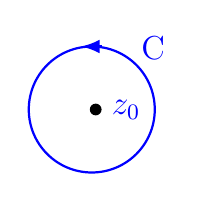
\begin{tikzpicture}[
    >=Latex, % Set default arrow tip style
    dot/.style={fill=black, circle, inner sep=1.5pt} % Style for z0 point
]

    % Define circle parameters
    \coordinate (Center) at (0,0);
    \def\radius{0.8};
    % Define z0 position slightly offset from center
    \coordinate (z0) at (0.05, -0.);

    % Draw the blue circle
    \draw[blue, thick] (Center) circle (\radius);

    % Draw the point z0 and its label
    % Make label large like the sketch
    \node[dot, label={[blue, font=\large]right:$z_0$}] at (z0) {};

    % Draw the counter-clockwise arrow near the top
    % Calculate point on circle at 90deg, then draw short arrow tangent-like
    \coordinate (ArrowPos) at ($(Center)+(90:\radius)$);
    % Adjust offsets to make arrow point left-to-right for CCW at top
    \draw[<-, blue, thick, shorten <=0.5pt, shorten >=0.5pt]
        ($(ArrowPos)+(-0.15,0)$) -- ($(ArrowPos)+(0.15,0)$);

    % Add the label C near the top right
    % Position relative to circle center using calc polar coordinates
    \node[blue, font=\large] at ($(Center)+(45:\radius+0.3)$) {C};

\end{tikzpicture}
\end{document}